% Chapter 4 -- Claim: Size and Value Explain Returns That Beta Cannot
% Figures need tikz and pgfplots (with the fillbetween library) in the preamble.
\providecolor{fenavy}{HTML}{1B2A6B}
\providecolor{fegray}{HTML}{4D4D4D}

\chapter{Claim: Size and Value Explain Returns That Beta Cannot}
\label{ch:04}

In the 1960s, finance seemed to have a complete answer to one of its oldest questions: why do some stocks earn more than others on average? The Capital Asset Pricing Model of Sharpe (1964) said that a stock's expected return depends on a single number, its beta with the market. The answer was elegant, and it was also bold, because it said exactly what should \emph{not} matter. A company's size, its price relative to its earnings or book value, and its own volatility should tell an investor nothing about its future return once beta is known. The early tests of Black, Jensen and Scholes (1972) and Fama and MacBeth (1973) found that returns did rise with beta, though less steeply than the theory said. Over the next decade, however, patterns appeared that the model said should not exist. Basu (1977) found that stocks with low price--earnings ratios earned more than their betas predicted, Banz (1981) found the same for small companies, and Rosenberg, Reid and Lanstein (1985) found it for stocks with high book-to-market ratios.

These findings mattered because of what they might mean. Fama (1970) had pointed out that market efficiency can only be tested together with a model of expected returns, so an anomaly always has two explanations: either the market misprices stocks, or the model of risk is wrong. The question came to a head when Fama and French (1992) showed that, once size and book-to-market were taken into account, beta had almost no power to explain average returns. Fama and French (1993) then proposed that size and value capture risks the market factor misses, and built the three-factor model on that idea. Lakonishok, Shleifer and Vishny (1994) offered the opposite reading: value stocks earn more because investors overreact to bad news and extrapolate past growth too far. The same numbers supported a story about risk and a story about mistakes.

The answer has large practical consequences. It decides what counts as skill when a fund manager beats the market, since a manager who simply holds small value stocks may earn a high CAPM alpha and no alpha at all against three factors. It affects the discount rate companies use for new projects (Graham and Harvey 2001), and it underpins the factor and smart-beta funds that now manage large sums for ordinary investors. As researchers have since proposed several hundred factors, the question has also become a statistical one: how many of these factors are real, and how many are the product of searching through the same data? The claim on trial\index{claims-on-trial method} in this chapter is therefore: \textbf{additional factors such as size and value explain differences in portfolio returns that beta cannot, but testing many candidate factors produces false discoveries, so a new factor must clear a higher bar.}

The chapter is built around Fama and French (1993, 2015), who showed that size, value, profitability and investment factors explain differences in returns that beta alone cannot. It also draws on Harvey, Liu and Zhu (2016), who warn that testing hundreds of candidate factors produces false discoveries. The lab in Section~\ref{sec:04-lab} replicates the Fama--French (1993) time-series regressions on their 25 size and book-to-market portfolios, in order to check whether the added factors really explain returns better than the CAPM, and then runs a factor-zoo experiment in order to see how many factors chance alone would appear to discover.

By the end of the chapter you will be able to:
\begin{itemize}
  \item summarize a return distribution by its mean, variance, skewness, kurtosis, and autocorrelation, and run and interpret a linear regression;
  \item explain why only systematic risk should earn a premium, and how a factor model turns that idea into a risk decomposition;
  \item trace the development of factor models from the CAPM, to the Fama--French three-factor model, to five- and six-factor models, and to the factor zoo, and interpret beta, alpha, and factor loadings at each step;
  \item execute a contemporaneous linear risk decomposition, partitioning total variance into systematic factor variance and idiosyncratic residual variance;
  \item test whether factors are priced with the GRS test and the Fama--MacBeth procedure;
  \item evaluate the practical and institutional implications of multi-factor architectures for asset management, style attribution, and corporate finance;
  \item explain what heteroskedasticity and serial correlation do to standard errors, and describe the stylized facts of financial returns: fat tails, volatility clustering, weak return autocorrelation, and asymmetry;
  \item choose standard errors that remain valid under these features: White, Newey--West (HAC), clustered, and Hodrick standard errors;
  \item use non-parametric block bootstrapping and Markov chain Monte Carlo (MCMC) simulations to measure uncertainty without relying on Gaussian assumptions;
  \item apply multiple-testing hurdles ($t > 3.0$) to prevent false discoveries in the factor zoo;
  \item separate statistical significance from economic significance.
\end{itemize}

In the lab you will replicate the main regressions of Fama and French (1993), decompose the risk of their 25 classic portfolios, measure the stylized facts of returns on real data, compute the portfolios' alphas under four standard error methods, and run a controlled experiment showing how overlapping long-horizon regressions find predictability that is not there.

\section{Foundations: Distributions and Regression}
\label{sec:04-foundations}

This section collects the two tools that the rest of the chapter builds on: the numbers that describe a single return series and the regression that links two series. Readers who know this material can skim it, but the notation introduced here is used throughout the book.

\subsection{Describing a Distribution}
Four numbers, called \textbf{moments}, summarize a return distribution:
\begin{itemize}
  \item The \textbf{mean}\index{mean} is its center: the average return.
  \item The \textbf{variance}\index{variance|textbf}, or its square root the standard deviation\index{standard deviation}, measures spread: how far returns typically fall from the mean.
  \item \textbf{Skewness}\index{skewness|textbf} measures asymmetry. It is negative when large losses are more likely than large gains of the same size, as for most stock indexes.
  \item \textbf{Kurtosis}\index{kurtosis|textbf} measures tail heaviness. A normal distribution has kurtosis 3; values above 3 indicate \textbf{fat tails}\index{fat tails|textbf}, meaning extreme returns occur far more often than a normal distribution predicts.
\end{itemize}

Figure~\ref{fig:04-moments} shows what each moment changes, by comparing the normal distribution with one that differs in that moment alone. The first two moments are the ones most investors already use: an average return and a volatility. The last two are the ones most often ignored, and they are the ones that matter most when markets turn violent. Two portfolios can have the same mean and the same standard deviation, yet one can lose 20\% in a day far more often than the other.

\begin{figure}[htbp]
\centering
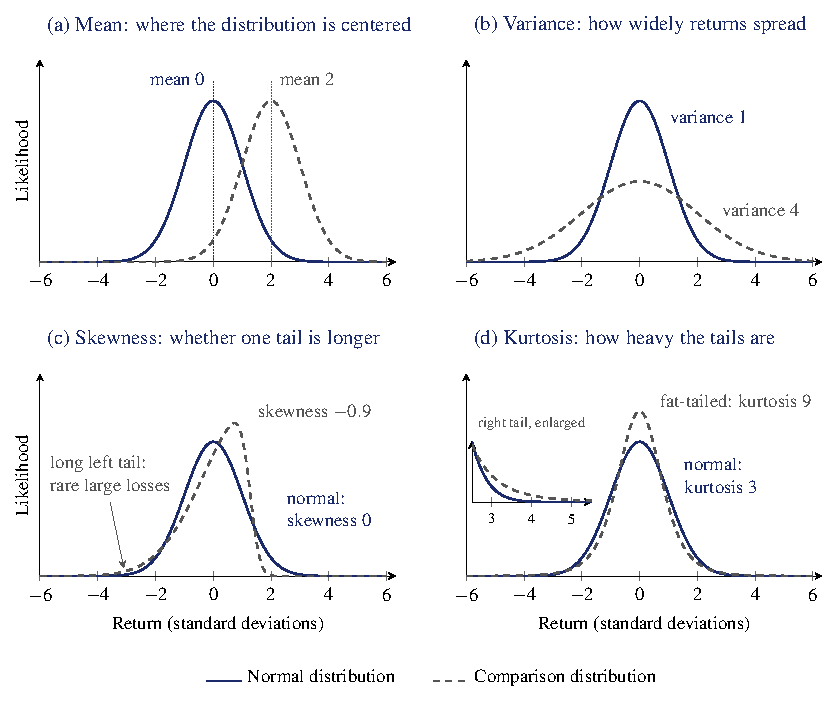
\includegraphics[width=0.7\linewidth]{images/fig03-0-moments.pdf}
\caption{The four moments of a distribution. Each panel compares the standard normal distribution (solid) with one that differs in a single respect. (a)~The mean sets the center. (b)~The variance sets the spread. (c)~Negative skewness lengthens the left tail, so large losses are more likely than large gains of the same size. (d)~Higher kurtosis puts more weight in the tails: the normal distribution has kurtosis 3, the fat-tailed one shown has kurtosis 9. Panels (c) and (d) keep the mean and variance of the normal distribution.}
\label{fig:04-moments}
\end{figure}

A fifth measure describes behavior over time. \textbf{Autocorrelation}\index{autocorrelation|textbf} is the correlation of a series with its own past values. The first-order autocorrelation ($\rho_1$) compares each month with the month before. A value near $+1$ means that a high month tends to be followed by another high month, a value near $-1$ means that it tends to be followed by a low month, and a value near zero means that the past says nothing about the next month. A return series with zero autocorrelation cannot be predicted from its own history.

\subsection{Linear Regression and OLS Assumptions}
\label{sec:04-regression}
A regression describes how a dependent variable, $y$, moves with an independent variable, $x$. Ordinary least squares\index{regression!ordinary least squares (OLS)} (OLS) fits
\begin{equation}
  y_t = \alpha + \beta x_t + \varepsilon_t
  \label{eq:04-ols}
\end{equation}
by choosing the intercept $\alpha$ and slope $\beta$ that minimize the sum of squared residuals $\sum \varepsilon_t^2$. The \textbf{residuals}\index{regression!residuals|textbf} $\varepsilon_t$ are the gaps between the actual values and the fitted line. The slope $\beta$ measures how much $y$ moves when $x$ moves by one unit, and the intercept $\alpha$ is the value of $y$ that the line predicts when $x$ is zero. The $R$-squared\index{regression!R-squared@$R^2$|textbf} ($R^2$) measures the share of the variance of $y$ explained by the regression, from 0 (none) to 1 (all).

A regression estimate also comes with a standard error, which measures how much the estimate would change if we drew a new sample. Chapter~\ref{ch:01} explained how standard errors are computed, and later chapters adjust them for features of financial returns such as fat tails and volatility clustering. This chapter focuses on what the estimates themselves mean.

% =====================================================================
% PART ONE OF THE CHAPTER: THE DEVELOPMENT OF RISK DECOMPOSITION
% =====================================================================
\section{Risk and Expected Return}
\label{sec:04-decomposition}


The Capital Asset Pricing Model (CAPM) provides a fundamental framework for understanding the relationship between risk and expected return. According to the CAPM, investors are compensated for bearing systematic market risk, which cannot be eliminated through diversification. 

However, empirical evidence suggests that market risk alone cannot fully explain the differences in average returns across stocks. In particular, researchers have documented persistent return patterns associated with firm size, book-to-market equity, profitability, and investment behavior.

To address these empirical patterns, researchers developed a series of multifactor asset pricing models that extend the traditional CAPM. The central economic idea is that \textbf{firms differ in their exposure to various sources of systematic risk and in their economic characteristics.} These differences may help explain why some groups of stocks earn higher average returns than others.


\subsection{The CAPM: One Source of Priced Risk}
\label{sec:04-capm}
The Capital Asset Pricing Model\index{capital asset pricing model (CAPM)} (Sharpe 1964, Lintner 1965, Mossin 1966) was the first formal risk decomposition, and it uses a single factor. It splits risk into two components. \textbf{Systematic risk}\index{risk!systematic|textbf} moves with the aggregate market and cannot be diversified away. \textbf{Idiosyncratic risk}\index{risk!idiosyncratic|textbf} is unique to individual assets and can be eliminated by holding a broad portfolio, a practice called \textbf{diversification}\index{diversification|textbf}. Because investors can remove idiosyncratic risk at almost no cost, the model says that they should not expect to be paid for bearing it. Only systematic risk earns a reward.

The CAPM says if every investor holds the market portfolio, then bad times are simply times when the market falls, and an asset's risk is measured by how much it falls along with the market. One number, the asset's sensitivity to the market, is then enough to set its expected return.


This one idea still underlies almost all of asset pricing, and its reach into practice is wide. Companies use the CAPM to set the discount rate\index{discount rate} for investment projects, and surveys find that most finance officers rely on it to estimate their cost of capital (Graham and Harvey 2001). The idea of alpha, the return beyond what market exposure explains, comes directly from the model, and its conclusion that the market portfolio is the best risky portfolio for every investor gave index funds their theoretical foundation.

Formally, the CAPM says that an asset's expected excess return\index{return!excess} is proportional to its \textbf{beta}\index{beta|textbf}, its sensitivity to the market:
\begin{equation}
  E[R^{e}_{i}] = \beta_i \, E[R^{e}_{m}], \qquad \beta_i = \frac{\operatorname{Cov}(R_i, R_m)}{\operatorname{Var}(R_m)}
  \label{eq:04-capm}
\end{equation}
Here $R_i$ is the asset's return, $R_m$ is the market's return and $R_f$ is the risk-free rate, so that $R^{e}_{i} = R_i - R_f$ and $R^{e}_{m} = R_m - R_f$ are their excess returns, as in Equation~\eqref{eq:excess-return}. The covariance $\operatorname{Cov}$ measures how two returns move together, and the variance $\operatorname{Var}$ measures how much one return moves on its own. A stock with a beta of 1.5 tends to rise 1.5\% when the market rises 1\%, so it carries one and a half times the market's systematic risk and should earn one and a half times the market's excess return.

The regression model is estimated in time series:
\begin{equation}
  R^{e}_{i,t} = \alpha_i + \beta_i R^{e}_{m,t} + \varepsilon_{i,t}
  \label{eq:04-capm-ts}
\end{equation}
This is Equation~\eqref{eq:04-ols} with the asset's excess return as $y$ and the market's excess return as $x$. The slope $\beta_i$ measures systematic market sensitivity. The intercept $\alpha_i$\index{alpha|textbf} (alpha) represents the average excess return that market exposure does not explain. The model predicts that $\alpha_i = 0$ for all assets, so a positive alpha is either evidence against the model or evidence of skill. Figure~\ref{fig:04-alpha} shows the two numbers on a scatter plot.

\begin{figure}[!htbp]
  \centering
  \begin{tikzpicture}[
    % Fitted regression: strategy = 1.16 + 1.15 * market
    declare function={fit(\x) = 1.16 + 1.15*\x;  zero(\x) = 1.15*\x;}
  ]
  \begin{axis}[
    scale only axis, width=0.41\linewidth, height=0.29\linewidth,
    axis lines=left,
    axis line style={-stealth, thin},
    xmin=-11, xmax=12.5, ymin=-12.5, ymax=16,
    xtick={-8,-4,0,4,8,12},
    ytick={-10,-5,0,5,10,15},
    tick label style={font=\footnotesize}, label style={font=\small},
    xlabel={Market excess return, $R^{e}_{m}$ (\% a month)},
    ylabel={Strategy excess return (\%)},
    clip=false,
  ]
    % Reference axes through zero
    \draw[gray!40] (axis cs:-11,0) -- (axis cs:12.5,0);
    \draw[gray!40] (axis cs:0,-12.5) -- (axis cs:0,16);

    % Monthly observations (illustrative)
    \addplot[only marks, mark=*, mark size=1.6pt, gray!60] coordinates {
      (0.51,2.80) (1.75,3.22) (-0.65,1.41) (-3.24,-0.57) (-1.41,-1.36)
      (-3.66,-2.80) (0.75,1.49) (6.13,8.66) (-1.57,-2.27) (-2.11,-2.05)
      (2.56,3.99) (2.00,4.86) (0.94,3.96) (-3.41,-4.63) (0.38,0.58)
      (3.42,6.19) (-5.15,-7.62) (-1.42,-1.08) (-7.49,-7.73) (-4.92,-2.80)
      (-7.24,-6.33) (-0.49,0.21) (-4.82,-4.97) (1.64,2.83) (1.16,4.75)
      (-0.29,0.31) (-10.07,-11.07) (-1.76,-0.34) (0.30,1.43) (0.98,2.12)
      (-5.93,-7.31) (-1.51,-0.55) (-3.61,-3.64) (-2.90,-0.54) (4.96,8.01)
      (-2.89,-2.20) (0.36,2.61) (4.21,5.75) (-1.95,0.41) (0.03,1.27)
      (0.96,3.20) (0.77,0.35) (-4.65,-3.75) (0.82,-0.15) (6.21,5.73)
      (-6.00,-6.26) (4.11,4.84) (1.00,2.66) (-2.19,1.80) (8.90,10.59)
      (3.70,4.74) (-4.54,-3.82) (0.81,2.90) (2.92,4.45) (-0.29,0.61)
    };

    % Zero-alpha line and fitted line
    \addplot[thick, dashed, fegray, domain=-11:12, samples=2] {zero(x)};
    \addplot[very thick, fenavy, domain=-11:12, samples=2] {fit(x)};
    \node[fenavy, anchor=west, font=\footnotesize] at (axis cs:12.3,{fit(12)+0.5}) {fitted line};
    \node[fegray, anchor=west, font=\footnotesize] at (axis cs:12.3,{fit(12)-3.5}) {zero-alpha line};

    % Slope triangle: run 3, rise 3 x beta
    \draw[fenavy] (axis cs:6,{fit(6)}) -- (axis cs:9,{fit(6)}) -- (axis cs:9,{fit(9)});
    \node[fenavy, anchor=north, font=\footnotesize] at (axis cs:7.5,{fit(6)-0.2}) {3};
    \node[fenavy, anchor=north west, font=\footnotesize, align=left] at (axis cs:9.3,{fit(6)-0.3})
      {rise $= 3\times$ beta\\beta $= 1.15$};

    % Alpha: the fitted line's value at a zero market return
    \fill[fenavy] (axis cs:0,1.16) circle (2.6pt);
    \draw[-stealth, fenavy] (axis cs:5.6,-3.4) -- (axis cs:0.4,0.9);
    \node[fenavy, anchor=north west, align=left, font=\footnotesize] at (axis cs:5.6,-2.6)
      {alpha $= 1.16$: the fitted line's\\value when the market return is 0};
  \end{axis}
  \end{tikzpicture}
\caption{Beta and alpha in a regression of a strategy's monthly excess returns on the market's. Beta is the slope of the fitted line; alpha is its height where the market's excess return is zero, the gap between the fitted line and a line with the same slope through the origin. Simulated data, with an alpha larger than any real strategy's so that it is visible.}
\label{fig:04-alpha}
\end{figure}

\textbf{The CAPM's variance decomposition.} Taking the variance of both sides of Equation~\eqref{eq:04-capm-ts} splits the asset's total risk into two parts. OLS makes the residuals uncorrelated with the market in the sample, so there is no cross term between them:
\begin{equation}
  \operatorname{Var}(R^{e}_{i}) = \beta_i^2 \operatorname{Var}(R^{e}_{m}) + \operatorname{Var}(\varepsilon_i)
  \label{eq:04-vardec-capm}
\end{equation}

Let's understand the two terms:
\begin{enumerate}
\item The first term is the \textbf{systematic variance}\index{variance!systematic|textbf}, the part that comes from exposure to the market, and 
\item the second is the \textbf{idiosyncratic variance}\index{variance!idiosyncratic|textbf}, the part that belongs to the asset alone. 
\end{enumerate}
The decomposition gives the regression's $R^2$ a direct economic meaning. The share of systematic variance in the total is exactly the $R^2$, so an $R^2$ of 0.9 says that 90\% of the asset's risk comes from the market and only 10\% is its own.

\begin{figure}[!htbp]
  \centering
  \begin{tikzpicture}[x=1cm, y=0.05cm]
    % Vertical axis: share of total variance, 0 to 100 percent
    \draw[-stealth, thin] (0,0) -- (0,108);
    \foreach \vdY in {0,50,100} {
      \draw (-0.08,\vdY) -- (0.08,\vdY);
      \node[anchor=east, font=\footnotesize] at (-0.1,\vdY) {\vdY};
    }
    \node[rotate=90, font=\small] at (-1.0,50) {Share of total variance (\%)};
    \draw[thin] (0,0) -- (6.6,0);

    % Bar 1: one stock, 31% systematic and 69% idiosyncratic
    \fill[fenavy!75] (0.8,0) rectangle (2.6,31);
    \fill[fenavy!15] (0.8,31) rectangle (2.6,100);
    \draw[fenavy] (0.8,0) rectangle (2.6,100);
    \node[white, font=\footnotesize, align=center] at (1.7,15.5) {systematic\\31\%};
    \node[fenavy, font=\footnotesize, align=center] at (1.7,65.5) {idiosyncratic\\69\%};
    \node[anchor=north, font=\small, align=center] at (1.7,-2) {One stock};

    % Bar 2: portfolio of 100 stocks, 98% systematic and 2% idiosyncratic
    \fill[fenavy!75] (3.8,0) rectangle (5.6,98);
    \fill[fenavy!15] (3.8,98) rectangle (5.6,100);
    \draw[fenavy] (3.8,0) rectangle (5.6,100);
    \node[white, font=\footnotesize, align=center] at (4.7,49) {systematic\\98\%};
    \draw[fenavy, thin] (5.6,99) -- (6.0,104);
    \node[fenavy, anchor=west, font=\footnotesize] at (6.0,104) {idiosyncratic 2\%};
    \node[anchor=north, font=\small, align=center] at (4.7,-2) {Portfolio of\\100 stocks};
  \end{tikzpicture}
  \caption{Splitting total variance into systematic and idiosyncratic parts with Equation~\eqref{eq:04-vardec-capm}. Each stock has a market beta of 1.2 and a residual standard deviation of 8\% a month, and the market's standard deviation is 4.5\% a month. Diversification leaves the systematic variance unchanged but divides the idiosyncratic variance by 100, so the systematic share, which equals the regression's $R^2$, rises from about 31\% to about 98\%. The numbers are illustrative.}
  \label{fig:04-vardec}
\end{figure}

The CAPM implies that a stock's expected return depends not on its total volatility, but on how sensitive it is to movements in the overall market. In practice, the CAPM provides a benchmark for determining the required return on investments, estimating the cost of equity capital for companies, evaluating portfolio performance, and making capital budgeting decisions. 

Empirical tests, however, show that the model fits the data less well than its influence suggests. If the CAPM were right, average returns would rise with beta along a straight line through the market portfolio, called the \textbf{security market line}\index{security market line|textbf}. Black, Jensen, and Scholes (1972) found that the security market line is flatter than predicted: low-beta stocks earn higher returns than the CAPM implies, while high-beta stocks earn lower returns (Figure~\ref{fig:04-sml}). 
The flatter security market line is important because it shows that the relationship between market risk and expected return is weaker than the CAPM predicts. In other words, low-beta stocks earn higher returns than the CAPM suggests, while high-beta stocks earn lower returns than expected. This means that taking on more market risk does not necessarily lead to proportionally higher returns. The finding challenges the CAPM's assumption that beta alone explains differences in expected returns and suggests that other factors may also influence stock performance. 

Later, Fama and French (1993) found that size and the book-to-market ratio\index{book-to-market ratio} explain differences in average returns that beta cannot. As a literal description of expected returns, the CAPM is therefore largely rejected, but it remains the benchmark against which every later model is built and tested. 
Interestingly, more research found that the stocks that the CAPM could not explain were not random. Their returns were related to certain company characteristics, such as size and book-to-market value. This suggested that factors beyond overall market risk also help explain why some stocks earn higher returns than others.




\begin{figure}[!htbp]
  \centering
  \begin{tikzpicture}[
    % CAPM security market line: E[R^e] = 8 * beta (% a year)
    % Illustrative empirical line, flatter: 3 + 3.5 * beta
    declare function={sml(\b) = 8*\b; emp(\b) = 3 + 3.5*\b;}
  ]
  \begin{axis}[
    scale only axis, width=0.43\linewidth, height=0.28\linewidth,
    axis lines=left,
    axis line style={-stealth, thin},
    xmin=0, xmax=1.95, ymin=0, ymax=15.5,
    xtick={0,0.5,1,1.5},
    ytick={0,4,8,12},
    xticklabel style={/pgf/number format/fixed},
    tick label style={font=\small}, label style={font=\small},
    xlabel={Beta, $\beta$},
    ylabel={Average excess return (\% a year)},
    clip=false,
  ]
    % CAPM prediction
    \addplot[fenavy, very thick, domain=0:1.85, samples=2] {sml(x)};
    \node[fenavy, anchor=west, font=\footnotesize] at (axis cs:1.86,{sml(1.85)}) {CAPM prediction};

    % Flatter line found in the data (illustrative)
    \addplot[fegray, thick, dashed, domain=0:1.85, samples=2] {emp(x)};
    \node[fegray, anchor=north west, font=\footnotesize] at (axis cs:1.86,{emp(1.85)+0.3}) {found in the data};

    % Ten beta-sorted portfolios (illustrative)
    \addplot[only marks, mark=*, mark size=1.8pt, fegray] coordinates {
      (0.55,5.1) (0.66,5.0) (0.76,5.9) (0.86,6.2) (0.95,6.1)
      (1.04,6.9) (1.14,6.7) (1.25,7.6) (1.37,7.5) (1.52,8.4)
    };

    % The market portfolio
    \fill[fenavy] (axis cs:1,8) circle (2.8pt);
    \node[fenavy, anchor=south east, font=\footnotesize] at (axis cs:0.97,8.2) {market};

    % Gap for high-beta stocks
    \draw[stealth-stealth, gray!70] (axis cs:1.6,{emp(1.6)}) -- (axis cs:1.6,{sml(1.6)});
    \node[anchor=west, font=\footnotesize, align=left] at (axis cs:1.63,11.8)
      {high-beta stocks earn\\less than predicted};
  \end{axis}
  \end{tikzpicture}
  \caption{The security market line. The CAPM predicts that average excess returns rise in a straight line with beta, passing through zero at a beta of zero and through the market's excess return at a beta of one (solid line). Tests that sort stocks into portfolios by beta typically find a flatter line with a positive intercept (dashed line and dots), so low-beta stocks earn more than predicted and high-beta stocks earn less (Black, Jensen and Scholes 1972). The numbers are illustrative.}
  \label{fig:04-sml}
\end{figure}

\subsection{The Three-Factor Model: Decomposing What the Market Leaves Behind}
\label{sec:04-factors}
To capture the return variation that market beta misses, Fama and French (1993) introduced the three-factor model\index{Fama--French factors}. It adds two long--short portfolios to the market:
\begin{itemize}
  \item $SMB$\index{factor!SMB (size)} (Small Minus Big) is the return of small stocks minus the return of large stocks;
  \item $HML$\index{factor!HML (value)} (High Minus Low) is the return of value stocks, which have high book-to-market ratios, minus the return of growth stocks, which have low ones.
\end{itemize}
The model is
\begin{equation}
  R^{e}_{i,t} = \alpha_i + b_i R^{e}_{m,t} + s_i \,\mathrm{SMB}_t + h_i \,\mathrm{HML}_t + \varepsilon_{i,t}
  \label{eq:04-ff3}
\end{equation}
where $b_i$, $s_i$, and $h_i$ represent the asset's systematic exposures to the three factors, called its \textbf{factor loadings}\index{factor!loadings|textbf}. A portfolio of small value stocks, for example, would have a positive $s_i$ and a positive $h_i$, while a portfolio of large growth stocks would have negative values for both.

Each factor is a \textbf{long--short} portfolio. 
A long--short portfolio involves buying stocks in one group and short-selling stocks in another. Buying stocks means the investor owns them and hopes their prices will rise. Short-selling means borrowing stocks and selling them, hoping to buy them back later at a lower price. For example, the SMB factor buys stocks of small companies and short-sells stocks of large companies. The goal is to profit when small-company stocks perform better than large-company stocks.

The beauty of the Fama--French SMB factor is that it captures the difference in returns between small and large companies through a simple long--short strategy. By buying small-company stocks and short-selling large-company stocks, it isolates the performance of smaller firms relative to larger ones. This approach allows investors to measure the size effect directly, without relying on the overall direction of the stock market.

\textbf{The economic argument.} Why should size and value earn premia? 
Fama and French offered a risk-based explanation. They argued that small companies and financially distressed companies face risks that are not fully captured by the overall market factor. Small companies tend to share common return movements that differ from those of large companies. Similarly, value companies, which often have persistently weak earnings, tend to be more financially distressed than growth companies. Their stock returns reflect this additional source of risk. Investors may therefore require higher expected returns to hold these stocks. In this interpretation, SMB and HML capture risks beyond the overall market risk.

\textbf{Alpha decay.} Moving from the CAPM to three factors does not remove any return; it relabels it. Returns that the CAPM counted as alpha are reassigned to exposures to $SMB$ and $HML$. For the 25 portfolios sorted on size and book-to-market, the $R^2$ rises substantially, above 90\% for most portfolios, and the alphas shrink toward zero (Fama and French 1993). This \textbf{alpha decay}\index{alpha!decay|textbf} is the main practical consequence of the new decomposition: a manager who looked skilled under the CAPM may simply have held small value stocks.


\subsection{Beyond Three Factors: The Fama--French Five-Factor Model}
\label{sec:04-multifactor}

The Fama--French three-factor model was later extended to include profitability and investment. These two additions were not entirely new
discoveries. They were motivated by earlier empirical studies showing that firms' profitability and investment decisions are related to
average stock returns. For example, Titman, Wei, and Xie (2004) found that firms with higher investment tend to earn lower subsequent
returns. Xing (2008) reported similar evidence. On the profitability side, Fama and French (2006) and Novy-Marx (2013) found that more
profitable firms tend to earn higher average returns. Building on this earlier research, Fama and French (2015) incorporated profitability
and investment into their existing three-factor model, creating the five-factor model.

The two new factors are \textbf{profitability} \index{factor!RMW (profitability)} ($RMW$, Robust Minus Weak) and
\textbf{investment}\index{factor!CMA (investment)} ($CMA$, Conservative Minus Aggressive). RMW measures the return difference between stocks of
highly profitable firms and those of less profitable firms. CMA measures the return difference between firms that invest conservatively
and those that invest aggressively. 

The five-factor model is:

\begin{equation}
  R^{e}_{i,t} = \alpha_i + b_i R^{e}_{m,t} + s_i \,\mathrm{SMB}_t + h_i \,\mathrm{HML}_t + r_i \,\mathrm{RMW}_t + c_i \,\mathrm{CMA}_t + \varepsilon_{i,t}
  \label{eq:04-ff5}
\end{equation}

Why should profitability and investment help explain stock returns? Fama and French (2015) state that a firm's value depends on its expected future cash flows and the return investors require.
Holding other things constant, firms with higher expected profitability should have higher expected returns. In contrast, firms that invest
more aggressively should have lower expected returns. 
Fama and French also found that, in their sample, the
HML factor added little explanatory power for average returns once profitability and investment were included. In other words, the
higher average returns of value stocks could largely be explained by their exposures to profitability and investment. This finding suggests
that the information captured by HML overlaps with that captured by RMW and CMA.

These extensions also change how we interpret alpha. Under the CAPM, alpha measures the return that cannot be explained by market risk.
Under the five-factor model, alpha measures the return that cannot be explained by market risk, size, value, profitability, and investment.
A different set of factors may produce a different alpha. Therefore, alpha is not simply a characteristic of an asset; it depends on the
asset pricing model used to evaluate it. Any discussion of alpha should make clear which model is being used.

\subsection{The Factor Zoo}
\label{sec:04-zoo}
The search did not stop at five or six factors. As Cochrane (2011) and Harvey, Liu, and Zhu (2016) document, intense backtesting has led to a ``zoo of factors''\index{factor zoo|textbf} comprising hundreds of published anomalies; Harvey, Liu, and Zhu counted more than 300. Each began life the same way as momentum and profitability did, as a pattern in average returns that the existing model could not explain.

Cochrane (2011) posed the question that the zoo raises: which characteristics really provide independent information about average returns, and which are the same few effects measured in different ways? The logic of risk decomposition offers one answer, and statistics offers another. The economic answer is that a factor deserves a place in the model only if there is a reason to expect its returns to track bad times, or a reason to expect a mispricing that arbitrage cannot remove. Without such a reason, adding factors becomes a mechanical exercise. Every new factor turns some alpha into beta, and with enough factors almost any alpha can be made to disappear, so the decomposition loses its power to tell skill from exposure.

The statistical answer is that a factor found by searching through hundreds of candidates must clear a higher bar than one proposed in advance. Most factors in the zoo were found by testing many candidate signals on the same few decades of U.S. data, which is exactly the kind of search that Chapter~\ref{ch:01} warned about. Section~\ref{sec:04-multiple-testing} explains why such a search demands strict multiple-testing corrections. The zoo is where the two halves of this chapter meet: the risk decomposition supplies the candidate factors, and the $t$-statistic decides which of them survive.

Although researchers have proposed more than 300 factors, these
factors do not represent 300 completely different sources of risk.
Many are closely related to one another or are alternative ways of
measuring similar firm characteristics and return patterns. For
example, several factors capture different aspects of value,
profitability, investment, or momentum. Others are variations of
existing factors that use different accounting measures, portfolio
construction methods, or sample periods. The factors listed in
Table~\ref{tab:04-factor-zoo} represent some of the major ideas
behind this large body of research. Understanding these broad
categories makes the factor zoo easier to navigate.

\begin{table}[htbp]
\centering
\caption{Selected Factors in Empirical Asset Pricing}
\label{tab:04-factor-zoo}
\small
\begin{tabularx}{\textwidth}{l l X l}
\hline
\textbf{Factor} & \textbf{Name} & \textbf{Economic meaning} & \textbf{Key study} \\
\hline
MKT & Market
& Excess return of the overall stock market over the risk-free rate.
& Sharpe (1964) \\

SMB & Size
& Small firms tend to earn higher average returns than large firms.
& Fama and French (1993) \\

HML & Value
& High book-to-market firms tend to earn higher average returns than low book-to-market firms.
& Fama and French (1993) \\

MOM & Momentum
& Stocks that performed well recently tend to continue outperforming recent losers.
& Jegadeesh and Titman (1993) \\

RMW & Profitability
& Firms with strong profitability tend to earn higher average returns than firms with weak profitability.
& Fama and French (2015) \\

CMA & Investment
& Firms that invest conservatively tend to earn higher average returns than firms that invest aggressively.
& Fama and French (2015) \\

LIQ & Liquidity
& Stocks with greater exposure to liquidity risk may earn higher returns.
& Pástor and Stambaugh (2003) \\

ACC & Accruals
& Firms with high accruals tend to earn lower subsequent returns than firms with low accruals.
& Sloan (1996) \\

IVOL & Idiosyncratic volatility
& Stocks with high idiosyncratic volatility tend to earn lower subsequent returns than stocks with low volatility.
& Ang et al. (2006) \\

BAB & Betting Against Beta
& Low-beta stocks tend to outperform high-beta stocks on a risk-adjusted basis.
& Frazzini and Pedersen (2014) \\
\hline
\end{tabularx}
\end{table}


\subsection{Statistical significance versus economic significance}
\label{subsec:04-statistical-economic-significance}

When researchers identify a factor with a positive average return, an important question is whether the estimated premium is statistically significant. Statistical significance helps determine whether the observed premium is likely to reflect more than sampling variation. However, it does not tell us whether the premium is large enough to matter economically.

Consider a factor with an estimated average monthly return of 0.20\%. If its standard error is sufficiently small, the estimated premium may be statistically significant. Yet an annualized premium of approximately 2.4\% may or may not be attractive, depending on the risk involved and the costs of implementing the strategy. By contrast, a factor with a larger estimated premium may have substantial uncertainty and fail to meet conventional significance thresholds.

A common way to summarize a factor's historical performance is to calculate its annualized average return and Sharpe ratio. If $\bar{f}$ denotes the average monthly factor return and $s_f$ its monthly standard deviation, the annualized quantities are
\begin{equation}
  \text{Annualized premium}=12\bar{f},
  \qquad
  \text{Annualized Sharpe ratio}
  =\sqrt{12}\frac{\bar{f}}{s_f}.
  \label{eq:04-factor-sharpe}
\end{equation}
These calculations provide a convenient summary of the factor's historical return and risk. They rely on standard annualization conventions and should be interpreted with care, particularly when returns exhibit serial correlation.

Economic significance requires a broader assessment than the size of an estimated premium or its $t$-statistic. A strategy may generate a statistically significant return before costs but become unattractive after accounting for transaction costs, portfolio turnover, liquidity constraints and the practical difficulty of implementing the strategy. The results may also depend on the sample period, portfolio construction method and assumptions about trading.

There is another important distinction. A factor's historical premium does not, by itself, establish why the premium exists. Under a risk-based interpretation, investors earn compensation for bearing systematic risks. Under other interpretations, the premium may reflect mispricing, investor behavior or limitations in the empirical model. Establishing a reliable economic explanation requires more than observing a positive average return.

For these reasons, evaluating a factor requires several complementary questions:

\begin{itemize}
  \item \textbf{Statistical significance:} Is the estimated premium sufficiently precise to distinguish it from zero?
  \item \textbf{Economic significance:} Is the premium large enough to matter relative to the risk taken?
  \item \textbf{Implementability:} Does the premium remain attractive after transaction costs, turnover and liquidity constraints?
  \item \textbf{Economic interpretation:} Is there a convincing explanation for why the factor should earn a premium?
\end{itemize}

These questions are especially important in empirical asset pricing, where researchers may examine hundreds of candidate factors. A statistically significant result can arise by chance, particularly when many hypotheses are tested. Even a factor that survives statistical scrutiny must still demonstrate economic relevance and practical value. A credible factor discovery should therefore combine statistical evidence, economic reasoning and realistic investment considerations.



\subsection{Practical and Institutional Implications}
\label{sec:04-implications}

Multi-factor models have changed how investors evaluate fund
performance, manage portfolios, and make corporate investment
decisions. Three applications illustrate their importance.

\textbf{Asset management and identifying manager skill.}
A fund's excess return can be divided into two parts: returns
explained by exposure to common risk factors and the additional
return, called alpha, that the factors cannot explain. Investors
can now obtain exposure to many of these factors at relatively
low cost through index funds and factor-based funds. Therefore,
when evaluating an active fund manager, investors want to know
whether the manager's performance comes from genuine investment
skill or simply from holding stocks with certain factor
characteristics. Carhart (1997) found that momentum exposure and
fund expenses explain much of the apparent persistence in mutual
fund performance. Fama and French (2010) also found that very few
fund managers consistently generate returns that are high enough
to cover their costs.

\textbf{Performance evaluation and investment style.}
Multifactor models also help investors understand how a fund
generates its returns. By comparing a fund's returns with those
of different investment style indexes, researchers can identify
whether the fund follows a growth, value, or other investment
strategy, even without examining its individual holdings.
Sharpe (1992) demonstrated this approach using style analysis.
Institutional investors also monitor a manager's factor exposures
over time to detect changes in investment strategy, known as
\textbf{style drift}\index{style drift|textbf}. For example, if a
fund described as a value fund gradually loses its exposure to
the HML factor, its actual investment style may no longer match
its stated strategy.

\textbf{Corporate finance and the cost of capital.}
Companies also use asset pricing models to estimate the cost of
equity, which helps them decide whether a proposed project offers
a sufficient expected return. While the CAPM uses only market
risk, multifactor models allow companies to consider additional
sources of risk, such as firm size and other characteristics.
However, the CAPM remains the most widely used approach in
corporate practice (Graham and Harvey 2001). More factors do not
necessarily produce more accurate estimates. Fama and French
(1997) found that estimates of industry costs of equity were
highly uncertain under both the CAPM and the three-factor model,
with standard errors exceeding 3\% per year. Thus, multifactor
models may provide additional information for investment
decisions, but they do not eliminate the difficulty of estimating
the cost of capital accurately.


\subsection{The Factor Zoo and the Multiple-Testing Problem}
\label{sec:04-multiple-testing}

The growing number of proposed risk factors raises an important
statistical question: how should we judge whether a newly discovered
factor is genuinely related to expected stock returns? Traditionally,
researchers often regard a $t$-statistic greater than approximately
2.0 as evidence of statistical significance at the 5\% level. This
convention is appropriate when testing a single hypothesis under the
usual statistical assumptions. However, asset pricing research
presents a different situation. Researchers have tested hundreds
of possible factors, often using overlapping data, similar
methodologies, and related measures of firm characteristics. When
so many hypotheses are tested, some will appear statistically
significant simply by chance.

Harvey, Liu, and Zhu (2016)
address this problem. They argue that the traditional significance
threshold is too low for a field in which researchers have tested
so many potential explanations for the cross-section of stock
returns. Their central message is that statistical significance
must be evaluated in light of the entire search process, not just
the final result reported in an individual paper.

\textbf{Why testing many factors creates a problem.}
To understand their argument, consider a simple example. Suppose
a researcher tests 100 factors, none of which has a genuine
relationship with expected returns. 

If each factor is tested
individually at the 5\% significance level, Assuming
the tests are independent, the probability of obtaining at least
one false positive is
\begin{equation}
  1-(1-0.05)^{100} \approx 99.4\%. \nonumber
\end{equation}

The probability of avoiding a false positive is 1-0.05 = 0.95. 
$0.95^{100}$ represents the probability that all 100 tests avoid false positives. 
Subtracting this probability from 1 gives \textbf{the probability of at least one false positive}, which is approximately 99.4\%.

In other words, when 100 independent factors, each with a true premium of zero, are tested at the 5\% significance level, 
there is approximately a 99.4\% 
chance that at least one will incorrectly appear to have a significant premium.

This issue is known as the \textbf{multiple-testing problem}.
\index{multiple-testing problem|textbf} A conventional $t$-test
evaluates one hypothesis at a time. It does not account for the
number of other hypotheses that researchers have examined.
Consequently, a factor with a $t$-statistic of 2.1 may appear
significant when considered in isolation, even though the result
is much less convincing after accounting for the many other
factors that researchers have tried.

There is another difficulty: researchers and academic journals
are more likely to report statistically significant findings than
unsuccessful experiments. A factor that produces a $t$-statistic
of 2.5 may be published, while another factor that produces a
$t$-statistic of 0.8 may never appear in a journal article. The
published literature therefore contains a disproportionate
number of successful results. This phenomenon is known as
\textbf{publication bias}\index{publication bias|textbf}. It
creates a form of selection bias: the factors we observe are
already those that have passed an initial significance threshold.

Harvey, Liu, and Zhu emphasize that the number of published
factors is not the same as the total number of factors researchers
have tested. The unsuccessful experiments that never become
publicly available are also part of the research process and
should be considered when evaluating the reliability of reported
discoveries.

\textbf{How many factors have researchers actually tested?}
To investigate the scale of the problem, Harvey, Liu, and Zhu
(2016) assembled a database of 313 research papers that proposed
and tested 316 factors related to the cross-section of expected
stock returns. 

The list of 316 factors illustrates the extensive search for
variables that can explain differences in average stock returns.
The 316 factors do
not necessarily represent 316 independent sources of risk.
But more importantly, the authors recognized that factors that failed to
produce significant results were unlikely to be published.
Their statistical framework therefore attempts to account for
these unobserved tests rather than treating the published
literature as the complete record of research activity.

The authors then evaluate how demanding the statistical
significance threshold should be when researchers test many
potential factors. They consider several approaches that
differ in how strictly they control the possibility of false
discoveries. 


After accounting for multiple testing, unpublished
experiments and correlations among factors, they find
that the required $t$-statistic varies with the statistical
method and assumptions. Some stricter approaches require
a value more than 3.92. Their widely cited recommendation,
however, is that a newly discovered factor should generally
have a $t$-statistic greater than 3.0.
The precise threshold is not a universal constant. It depends
on the number of tests, the dependence among test statistics,
the assumed number of unreported experiments, and the chosen
error-control procedure. 

\subsection{Economical magnitude}
A statistically significant result is also not the same
as an economically important result. A factor may have a
high $t$-statistic but a very small average return, making
its practical investment value limited. Conversely, a
factor with an economically meaningful estimated premium
may not be statistically precise. Statistical significance,
economic magnitude, and a sound economic explanation
should therefore be considered together.

Finally, multiple-testing adjustments do not replace
careful empirical methods. Harvey, Liu, and Zhu take the
reported $t$-statistics as given and assume that the
underlying studies have appropriately addressed issues
such as heteroskedasticity, autocorrelation, and data
errors. 

\section{What Investors Can Use}
\label{sec:04-investors}

Most investors will never compute a Newey--West standard error or a GRS statistic, but the ideas in this chapter translate directly into questions about any statistical claim.

\textbf{Rules of Thumb:}
\begin{enumerate}
  \item \textbf{Unbundle alpha from factor beta.} Do not pay active fees for static loadings on known factors ($SMB$, $HML$, $UMD$), because those exposures can be bought cheaply through index and factor funds.
  \item \textbf{Count independent observations.} $T$ monthly observations with a $k$-month horizon provide only about $T/k$ independent periods. Fifty years of five-year returns is ten independent observations, not six hundred.
  \item \textbf{Demand higher cutoffs.} Require $t > 3.0$ for proposed factor anomalies to adjust for search bias, and remember that across 25 portfolios one or two will look significant by chance.
  \item \textbf{Convert $t$-statistics to net returns.} Evaluate alpha after transaction costs, short-selling fees, and turnover. A significant alpha smaller than the fund's fee is worth nothing to the investor.
\end{enumerate}

\textbf{Questions to Ask Fund Managers:}
\begin{itemize}
  \item What standard errors were used, and do your results hold under Newey--West HAC and block bootstrap methods?
  \item What fraction of net performance comes from true alpha versus systematic factor exposures?
  \item How many candidate models or variations were backtested before selecting this strategy?
  \item If you forecast over long horizons, how many non-overlapping periods does your sample contain?
  \item What is the confidence interval for your alpha, and how large is it after fees and trading costs?
\end{itemize}

\section*{Exercises}
\addcontentsline{toc}{section}{Exercises}

\subsection*{Conceptual (all readers)}
\begin{enumerate}
  \item An active equity manager reports a CAPM alpha of 3.2\% per year ($t = 2.5$). Under a Fama--French three-factor model, the alpha drops to 0.1\% ($t = 0.2$), with an $SMB$ loading of 0.70 and an $HML$ loading of 0.50. Explain the source of the manager's excess return, and what it implies for the fee the manager should charge.
  \item A stock has a market beta of 0.8, a residual standard deviation of 6\% a month, and the market's standard deviation is 4.5\% a month. Use Equation~\eqref{eq:04-vardec-capm} to compute the share of its variance that is systematic. What would the share be for an equally weighted portfolio of 50 such stocks with independent residuals?
  \item Fama and French (2015) found that the value factor becomes redundant once profitability and investment factors are added. Using the dividend discount model argument of Section~\ref{sec:04-multifactor}, explain why value stocks might load on these two factors, and discuss what the finding implies for reading $HML$ as a distress factor.
  \item Explain why adding factors to a model can always make an alpha smaller, and state what economic and statistical evidence you would require before accepting a newly proposed factor.
  \item Daily returns show minimal autocorrelation, yet absolute daily returns show strong autocorrelation. Explain how both statements can be true, and why this matters for standard errors.
  \item A long-horizon regression of 5-year returns on dividend yields uses 50 years of monthly data ($T=600$, $k=60$). How many independent observations does it contain, and why are classical $t$-statistics misleading?
  \item Why must a time-series bootstrap resample blocks of observations rather than individual months?
  \item Explain why a factor alpha with $t = 3.2$ might lack economic significance, and list what you would need to know before investing in it.
\end{enumerate}

\subsection*{Lab Extensions (technical readers)}
\begin{enumerate}
  \setcounter{enumi}{8}
  \item Replicate Part B of Lab~\ref{ch:04} across two sub-samples: 1963--1992 and 1993--present. Compare changes in factor risk premia and GRS test rejections.
  \item Compute $t$-statistics for 25 portfolio alphas using four methods: Classical OLS, White, Newey--West, and Stationary Block Bootstrap. Identify portfolios with the largest SE discrepancies, and explain what features of their returns might cause them.
  \item Pair monthly returns with 1,000 simulated non-predictive predictors ($\rho = 0.98$). Run long-horizon regressions ($k=1$ to $60$) and plot false-positive rates for OLS, Newey--West, and Hodrick standard errors. Then set the correlation between predictor shocks and return shocks to $-0.9$ and describe how the Stambaugh bias changes the results.
\end{enumerate}

\section{Lab~\thechapter: Replicating Fama and French (1993) and the factor zoo}
\label{sec:04-lab}

\begin{callout}
\textbf{Lab~\ref{ch:04} at a glance.} \emph{Papers replicated:} the time-series regressions of Fama and French (1993) on their 25 portfolios; a multiple-testing experiment after Harvey, Liu and Zhu (2016). All data are free. \emph{Claim on trial:} additional factors improve our ability to explain differences in portfolio returns, but testing many candidate factors can produce false discoveries. \emph{Data:} monthly returns on the 25 Fama--French portfolios formed on size and book-to-market, together with the market, size and value factors, from the Kenneth R. French Data Library\index{Kenneth French data library}. \emph{Tools:} Python with pandas, NumPy, SciPy and matplotlib, plus the fintest module. \emph{Time:} about two hours, including the guided notebook. \emph{Code:} repository folder \texttt{ch03-multifactor-models/}.
\end{callout}

This lab examines two important questions in empirical asset pricing. First, do additional risk factors improve our ability to explain stock returns? Second, when researchers test hundreds of potential factors, how can we distinguish genuine discoveries from results that arise by chance?

Part~A replicates the central empirical analysis of Fama and French (1993), using the 25 portfolios formed on size and book-to-market to estimate the CAPM and the Fama--French three-factor model. Readers compare the explanatory power and estimated factor exposures of the two models. Part~B conducts a controlled multiple-testing experiment inspired by Harvey, Liu and Zhu (2016), demonstrating why conventional significance thresholds can produce many false discoveries when researchers examine a large number of candidate factors. Part~C examines the economic significance of factor premiums and considers whether statistically significant results translate into attractive investment opportunities.

\subsection*{Part A: Replicating the Fama--French three-factor model}

The 25 portfolios formed on size and book-to-market are the classic \textbf{test assets}\index{factor!test assets|textbf} of Fama and French (1993): the portfolios whose returns an asset-pricing model is designed to explain. The lab uses monthly data beginning in July 1963 and estimates two models for each portfolio.

The first is the CAPM:
\begin{equation}
  R^{e}_{i,t}
  = \alpha_i+\beta_{i,M}R^{e}_{m,t}+\varepsilon_{i,t}.
  \label{eq:04-lab-capm}
\end{equation}

The second is the Fama--French three-factor model:
\begin{equation}
  R^{e}_{i,t}
  = \alpha_i+\beta_{i,M}R^{e}_{m,t}
  +\beta_{i,S}SMB_t
  +\beta_{i,H}HML_t+\varepsilon_{i,t},
  \label{eq:04-lab-ff3}
\end{equation}
where $R^{e}_{m,t}$ is the market excess return, which the French library labels Mkt-RF, $SMB$ is the return on small stocks minus large stocks, and $HML$ is the return on high book-to-market stocks minus low book-to-market stocks.

For each portfolio, the lab reports the estimated alpha, factor loadings and $R^2$. Readers then compare the results from the two models. Adding $SMB$ and $HML$ should improve the model's ability to explain the returns of portfolios formed on size and book-to-market. The estimated factor loadings also reveal how different portfolios are exposed to market, size and value risks.

The results illustrate an important distinction. A higher $R^2$ means that the model explains more of the variation in portfolio returns. It does not necessarily mean that the model fully explains differences in average returns or that every estimated alpha is zero. The estimated alphas provide an additional way to examine the returns that remain unexplained by the included factors.

\subsection*{Part B: A multiple-testing experiment}

The factor zoo creates a different statistical problem. If researchers test enough candidate factors, some will appear significant simply by chance, even when none has a genuine return premium.

To see why, consider 1,000 candidate factors, each of which has a true expected premium of zero. The lab simulates monthly returns for these factors and tests whether the average premium of each factor differs from zero. Because the true premium is known to be zero, every rejection is a false discovery.

The experiment applies two significance thresholds:
\begin{itemize}
  \item The conventional threshold, $|t|>1.96$, corresponding approximately to a two-sided 5\% test.
  \item A more demanding threshold, $|t|>3.0$, inspired by the recommendations of Harvey, Liu and Zhu (2016).
\end{itemize}

The lab repeats the experiment and records the number of false discoveries under each threshold. With 1,000 independent tests and a conventional 5\% significance level, we would expect approximately 50 false positives on average, even though none of the factors has a genuine premium. A higher threshold substantially reduces this number.

This experiment illustrates the basic logic behind the multiple-testing problem. The more candidate factors researchers examine, the greater the chance that some will appear significant by coincidence. Harvey, Liu and Zhu (2016) argue that the conventional $t$-statistic threshold of approximately 2 is too weak for many new factor discoveries and that a higher hurdle is needed.

The simulation is deliberately simplified: it treats the candidate factors as independent and assumes that their true premiums are zero. In actual asset-pricing research, candidate factors may be correlated, and some may have genuine economic foundations. The experiment is therefore not a replication of Harvey, Liu and Zhu (2016), but a demonstration of the statistical problem that motivates their analysis.

\subsection*{Part C: Statistical and economic significance}

A factor can have a statistically significant premium without offering an attractive investment opportunity. The final part of the lab examines the size of the estimated factor premiums and their potential economic value.

For each factor, the lab calculates its average monthly return, annualized premium and annualized Sharpe ratio. For a factor with monthly mean return $\bar{f}$ and standard deviation $s_f$, the annualized quantities are
\begin{equation}
  \text{Annualized premium}=12\bar{f},
  \qquad
  \text{Annualized Sharpe ratio}
  =\sqrt{12}\frac{\bar{f}}{s_f}.
  \label{eq:04-lab-sharpe}
\end{equation}

Readers then consider whether the estimated premiums are large enough to matter in practice. A strategy may have a statistically significant premium but require frequent trading, substantial turnover or investment in illiquid stocks. Transaction costs and implementation constraints can reduce or eliminate its apparent advantage.

The purpose is not to decide whether every factor is investable. Rather, it is to recognize that statistical evidence is only one part of evaluating an investment strategy. A credible finding should also have an economically meaningful magnitude and remain attractive after realistic implementation costs are considered.

\emph{[Draft note: the regression results and factor-premium estimates are generated from the Kenneth R. French Data Library at the time of publication. The multiple-testing experiment uses simulated data with known zero premiums. The book prints the numerical results; the accompanying notebook allows readers to reproduce the analysis.]}

\subsection*{Your verdict}

Readers judge the claim by comparing the results from all three parts. The expected verdict is \textbf{survives, with conditions}. The Fama--French three-factor model should explain more of the variation in the 25 size-and-book-to-market portfolios than the CAPM. Its additional factors capture systematic differences in portfolio returns that the market factor alone does not explain. However, a higher $R^2$ does not guarantee that all pricing errors disappear or that the model fully explains differences in expected returns.

The multiple-testing experiment reveals a separate limitation. When researchers examine hundreds of candidate factors, conventional significance thresholds can produce many false discoveries. A more demanding statistical hurdle helps, but it does not replace economic reasoning, theoretical motivation or out-of-sample validation.

Finally, statistical significance does not guarantee economic value. Factor premiums must be large enough to matter after considering risk, transaction costs and implementation constraints. The broader lesson is that a convincing factor discovery requires more than a significant $t$-statistic: it should help explain return differences, withstand appropriate statistical scrutiny and make economic sense.
